\documentclass[11pt, a4paper]{article}

\usepackage{listings}
\usepackage{color}
\usepackage[normalem]{ulem}
\usepackage{graphicx}

\definecolor{dkgreen}{rgb}{0,0.6,0}
\definecolor{gray}{rgb}{0.5,0.5,0.5}
\definecolor{mauve}{rgb}{0.58,0,0.82}

\lstset{frame=tb,
  language=SQL,
  aboveskip=3mm,
  belowskip=3mm,
  showstringspaces=false,
  columns=flexible,
  basicstyle={\small\ttfamily},
  numbers=none,
  numberstyle=\tiny\color{gray},
  keywordstyle=\color{blue},
  commentstyle=\color{dkgreen},
  stringstyle=\color{mauve},
  breaklines=true,
  breakatwhitespace=true
  tabsize=3
}

\begin{document}
\title{}
\author{Groep A\\ Rapport 1}
\date{19 maart 2014}
\maketitle


\section{Status}
De website staat momenteel nog niet online, maar de locale versie werkt wel al.	Veel, maar nog niet alle pagina's zijn al beschikbaar. Er kunnen ook al accounts aangemaakt worden en inloggen is mogelijk. De features voor ingelogde gebruikers zijn echter nog niet ge\"implementeerd. Merk op dat niet elke knop op de website al werkt!

\section{Taakverdeling}
\subsection{Stijn}
Ging op zoek naar verschillende bronnen voor data. Zocht uit hoe een web crawler nu precies werkt en programmeerde er zelf een specifiek voor onze doeleinden.
\subsection{Kristof}
Werkte het door iedereen samen opgestelde databaseschema af. Maakte heel wat webpagina's aan. Assisteerde Tom bij het voorspellingsalgoritme.
\subsection{Tom}
Werkte aan het voorspellingsalgoritme. Assisteerde Kristof bij het aanmaken van webpagina's.
\subsection{Jakob}
Bouwde het loginsysteem. Bouwde een klasse die het inserten van data in de database encapsuleert.
\subsection{Ruben}
Maakte een template voor de wepagina's. Converteerde iedereens code naar een mooie MVC-structuur om de code flexibeler en makkelijker leesbaar te maken en bracht andere verbeteringen aan in de code.

\section{Design}
De meesten van ons groepje hadden totaal geen ervaring met het bouwen van websites. In het begin van het project zijn de meesten dus begonnen met het doornemen van allerlei tutorials. Dit nam redelijk wat tijd in beslag, waardoor het eigenlijke project met wat vertraging begon. In eerste geval werkten we aan de backend van de website: opstellen van databaseschema, bouwen van loginsysteem, ... We waren eerst van plan om onze data te verkrijgen via de OpenFooty API. Ongeveer een week na het versturen van onze API key request begonnen we te vrezen dat we deze niet meer gingen krijgen, wat inderdaad nog steeds niet gebeurd is. We moesten dus op zoek gaan naar andere manieren om onze data te vergaren. De enige andere optie leek het gebruik van een crawler. Niemand van ons had enige ervaring met het schrijven/gebruiken van crawlers, en de crawler bleek een struikelblok. Ondertussen werkt de crawler min of meer, maar hij is nog niet in een ver genoeg stadium om data te verzamelen die compleet genoeg is om nuttig te zijn. We werken momenteel dus nog met manueel ingevoerde testdata. Ons voorspellingsalgoritme is al uitgedacht maar nog niet ge\"implementeerd. Verder zijn al sommige, maar niet alle webpagina's aangemaakt en is er een (tijdelijke?) vormgeving van de pagina's.
\\
\\
\\
Het voorspellingssysteem hebben wij opgesplitst in 2 essenti\"ele delen, namelijk het voorspellen van een winnaar van een wedstrijd, en het bepalen van de te verwachten score. Factoren die wij belangrijk vonden om rekening mee te houden in het voorspellen van dit alles zijn vooral onderlinge resultaten van eerder gespeelde wedstrijden, en gemiddeldes van andere wedstrijden tegen andere ploegen. Ook wordt altijd rekening gehouden met de locatie waar gespeeld wordt (uit of thuis).
\\
\\
Het voorspellen van de winnaar is natuurlijk de makkelijkste van de twee. We beginnen simpelweg door te kijken naar eerder gespeelde wedstrijden tussen deze ploegen. We werken met een puntensysteem waarbij een ploeg punten krijgt wanneer het een wedstrijd wint. Het aantal punten die ze krijgen, hangt af van de impact die we willen dat het heeft op het gehele resultaat. Hierbinnen maken we ook nog eens het onderscheid of de set-up uit/thuis dezelfde is of omgekeerd. Het eerste geval is natuurlijk het belangrijkste aangezien dit een identieke case is. Daarom zal een ploeg ook de meeste punten worden toegekend voor het winnen van zulke wedstrijden.
Daarna gaan we kijken naar algemene resultaten, maar weer rekening houdende met het al dan niet uit/thuis spelen. We kijken naar alle wedstrijden die de thuisploeg thuis speelde, en de uitploeg uit speelde. Voor elke gewonnen match krijgen ze ieder weer een bepaald aantal punten (afhankelijk van de impact die deze factor moet hebben). Vervolgens kijken we naar de wedstrijden waar de thuisploeg uit speelde, en de uitploeg thuis. Wederom krijgen ze voor iedere gewonnen match een bepaald aantal punten maar weer minder dan in het vorige geval. Tot slot gaan we de punten vergelijken en op basis daarvan kunnen we de kans bepalen dat een bepaalde ploeg wint.
\\
\\
Het bepalen van een score is iets complexer. Dit volgt een gelijkaardig systeem als hierboven, maar met een belangrijk verschil. Hier werken we niet met het optellen van punten. We gaan altijd werken met gemiddeldes. Zo zullen we wederom eerst kijken naar identieke wedstrijden en van elke ploeg het gemiddelde aantal goals bewaren. Dan gaan we kijken naar wedstrijden met dezelfde ploegen maar op een andere locatie en wederom berekenen we het gemiddeld aantal goals gescoord door de teams.
Dan gaan we weer kijken naar de algemene resultaten waarbij we wel wederom een onderscheid maken tussen uit- en thuis spelen. We berekenen dus het gemiddelde aantal goals dat de thuisploeg thuis scoort, en het gemiddelde aantal goals dat de thuisploeg uit scoort. Voor de uitploeg natuurlijk net hetzelfde. Nu zitten we met 4 gemiddeldes die we individueel vermenigvuldigen met een factor (mate van impact) en daarna optellen en delen door 4. Door dit af te ronden hebben we nu een aantal goals bepaald voor iedere ploeg. Maar hier liep het soms nog mis. Afhankelijk van de data kon de kans dat ploeg A won 90\% zijn maar de score berekenen in het voordeel van ploeg B.
Daarom checken we op het einde de kans op winst van een ploeg en passen de score indien nodig aan zodat deze uitkomt met de verwachte uitslag van de wedstrijd.
\\
\\
Ter uitbreiding zouden we graag nog meer data bepaald laten worden door het voorspellingsysteem. Dit zou dan eventuele spelers die scoren, kaarten, minuten van de goals, enzovoort zijn. Hiervoor moeten we echter eerst grondig de data die we ter beschikking hebben analyseren, en zo een geschikt algoritme hiervoor uitdenken dat hoogstwaarschijnlijk in dezelfde trend zal liggen als die hierboven.



\section{Database}
Onze database bestaat 12 tabellen met voetbalgerelateerde data en 1 tabel voor users.
\begin{enumerate}
\item 'continent': Tabel voor werelddelen. Bevat een id en een naam.
\item `country`: Tabel voor landen. Bevat een id, een naam, de id van het werelddeel waarin het land ligt, en een afkorting voor de naam van het land. Die afkorting zal gebruikt worden op de website.
\item `player`: Tabel voor voetbalspelers. Bevat een id, een naam en een boolean die aangeeft of de speler geblesseerd is.
\item `coach`: Tabel voor voetbalcoaches. Bevat een id en een naam.
\item `team`: Tabel voor voetbalteams. Bevat een id, een naam, een id van het land van het team, een id van de huidige coach van het team en de FIFA score.
\item `competition`: Tabel voor voetbalcompetities. Bevat een id en een naam.
\item `match`: Tabel voor voetbalmatches. Bevat id's van thuis- en uitteam, id van de competitie en een datum.
\item `playerPerTeam`: Tabel die spelers en teams met elkaar linkt. Bevat id's van een speler en een team.
\item `playerPerMatch`: Tabel die spelers en matches met elkaar linkt. Bevat id's van een speler en een match en de tijden waarop de speler op het veld kwam en van het veld ging.
\item `teamPerCompetition`: Tabel die teams en competities met elkaar linkt. bevat id's van een team en een competitie.
\item `goal`: Tabel voor doelpunten. Bevat id van match waarin doelpunt gescoord is, tijdstip waarop, id van de speler die het doelpunt scoorde, id van het team waarnaar het punt ging en een boolean die aangeeft of het doelpunt tijdens de penaltyfase gescoord werd.
\item `cards`: Tabel voor gele en rode kaarten. Bevat een id,	een id van de speler die de kaart kreeg, een id van de match waarin de kaart gegeven werd, de kleur van de kaart en de tijd waarop de kaart gegeven werd.
\end{enumerate}

\subsection{ER-diagramma}
Zie laatste pagina
\subsection{Relational model}
continent(\uline{id}, name) \\
country(\uline{id}, name, continent\_id, abbreviation) \\
player(\uline{id}, name, injured) \\
coach(\uline{id}, name) \\
team(\uline{id}, name, country\_id, coach\_id, fifascore) \\
competition(\uline{id}, name) \\
match(\uline{id}, hometeam\_id, awayteam\_id, competition\_id, date) \\
playerPerTeam(\uline{player\_id}, \uline{team\_id}) \\
playerPerMatch(\uline{player\_id}, \uline{match\_id}, intime, outtime) \\
playerPerCompetition(\uline{team\_id}, \uline{competition\_id}) \\
goal(match\_id, time, player\_id, team\_id, penaltyphase) \\
cards(\uline{id}, player\_id, color, time) \\

\subsection{Constraints}
\begin{lstlisting}
-- Constraints for table `cards`
--
ALTER TABLE `cards`
  ADD CONSTRAINT `match` FOREIGN KEY (`match_id`) REFERENCES `match` (`id`) ON DELETE NO ACTION ON UPDATE CASCADE,
  ADD CONSTRAINT `player` FOREIGN KEY (`player_id`) REFERENCES `player` (`id`) ON DELETE CASCADE ON UPDATE CASCADE;

--
-- Constraints for table `country`
--
ALTER TABLE `country`
  ADD CONSTRAINT `continent` FOREIGN KEY (`continent_id`) REFERENCES `continent` (`id`);

--
-- Constraints for table `goal`
--
ALTER TABLE `goal`
  ADD CONSTRAINT `goal_match` FOREIGN KEY (`match_id`) REFERENCES `match` (`id`) ON DELETE NO ACTION ON UPDATE CASCADE,
  ADD CONSTRAINT `goal_player` FOREIGN KEY (`player_id`) REFERENCES `player` (`id`) ON DELETE NO ACTION ON UPDATE CASCADE,
  ADD CONSTRAINT `goal_team` FOREIGN KEY (`team_id`) REFERENCES `team` (`id`) ON DELETE NO ACTION ON UPDATE CASCADE;

--
-- Constraints for table `match`
--
ALTER TABLE `match`
  ADD CONSTRAINT `awayteam` FOREIGN KEY (`awayteam_id`) REFERENCES `team` (`id`) ON DELETE CASCADE ON UPDATE CASCADE,
  ADD CONSTRAINT `hometeam` FOREIGN KEY (`hometeam_id`) REFERENCES `team` (`id`) ON DELETE CASCADE ON UPDATE CASCADE,
  ADD CONSTRAINT `match_competition` FOREIGN KEY (`competition_id`) REFERENCES `competition` (`id`);

--
-- Constraints for table `playerPerMatch`
--
ALTER TABLE `playerPerMatch`
  ADD CONSTRAINT `player_per_match` FOREIGN KEY (`match_id`) REFERENCES `match` (`id`) ON DELETE CASCADE ON UPDATE CASCADE;

--
-- Constraints for table `playerPerTeam`
--
ALTER TABLE `playerPerTeam`
  ADD CONSTRAINT `player_per_team` FOREIGN KEY (`team_id`) REFERENCES `team` (`id`) ON DELETE CASCADE ON UPDATE CASCADE;

--
-- Constraints for table `team`
--
ALTER TABLE `team`
  ADD CONSTRAINT `team_coach` FOREIGN KEY (`coach_id`) REFERENCES `coach` (`id`) ON DELETE NO ACTION ON UPDATE CASCADE,
  ADD CONSTRAINT `team_country` FOREIGN KEY (`country_id`) REFERENCES `country` (`id`);

--
-- Constraints for table `teamPerCompetition`
--
ALTER TABLE `teamPerCompetition`
  ADD CONSTRAINT `tpc_competition` FOREIGN KEY (`competition_id`) REFERENCES `competition` (`id`);

\end{lstlisting}

\section{User interface}

Hoewel Laravel beschikt over een volledig uitgewerkt loginsysteem, besloten we ons eigen systeem te schrijven. Een dergelijk systeem gebruikt een database voor het opslaan van users, dus is het niet meer dan logisch dat we dit in een vak met betrekking tot databases zelf gaan programmeren. In de database bestaat een tabel 'user', met als fields 'id', 'username', 'firstname', 'lastname', 'email', 'password', 'country', 'session\_id' en 'registrationcode'. De id is een auto incrementing integer die dient als key voor elke entry van de tabel. We voorzien een username, aangezien dit gebruikers een zekere vorm van anonimiteit biedt op onze website. Daarnaast is het een makkelijke manier om gebruikers op de website een unieke benaming te geven. Voornaam en familienaam zijn apart opgeslagen, zodat we in bijvoorbeeld emails gebruikers niet altijd met hun volledige naam niet hoeven aan te spreken. Het paswoord is uiteraard gehasht opgeslagen. Het hashen gebeurt via Laravel, aan de hand van bcrypt. Bcrypt is gebaseerd op het Blowfishalgoritme en heeft een salt ingebouwd, wat accounts beschermt tegen aanvallen gebruik makende van rainbow tables. Laravel biedt een functie voor het vergelijken van een ongehasht en gehasht paswoord. We vragen gebruikers ook in welk land ze wonen, zo kunnen we bijvoorbeeld bepaalde competities en nieuwsberichten een prominentere plek op de website geven afhankelijk van de gebruiker. De session\_id wordt gebruikt om bij te houden of een gebruiker ingelogd is. We plaatsen een tijdelijke cookie met hetzelfde id bij de gebruiker, en kunnen dit zo nagaan. Ten slotte wordt de registratiecode gebruikt bij het nagaan van de validiteit van het emailadres van een gebruiker. De registratiecode wordt gemaild naar de gebruiker, en het account wordt pas geactiveerd wanneer deze code ingegeven wordt. Merk op dat deze functionaliteit momenteel nog niet actief is, gezien we nog niet beschikken over een mailserver.
\\
\\
Voor de validatie van input bij registreren (zijn verplichte velden ingevuld, staat bij emailadres wel een emailadres, is tweemaal hetzelfde paswoord ingetypt, ...) is de validatie van Laravel gebruikt. Dergelijke validatiecode ziet er heel wat beter uit voor de programmeur dan via een hoop simpele if-statements en reguliere expressies. We gebruiken de prepared statements van Laravel om sql-injecties tegen te gaan. Verder gebruiken we de Laravel Query Builder voor makkelijker schrijven van SQL queries niet, dit gebeurt zoals opgegeven met ruwe SQL queries.
\\
\\
Op elke webpagina verschijnt voor een niet-ingelogde gebruiker een loginknop. Het loginmenu wordt dan over de huidige pagina weergegeven. Daar is ook een "forgot password"-functionaliteit voorzien. De gebruiker geeft of zijn username of zijn emailadres in, en er wordt een email gestuurd waarmee het paswoord gereset kan worden. Wederom, deze functionaliteit is nog niet actief. Bij een ingelogde gebruiker wordt bij elke bezochte pagina de login cookie gerefresht, zodat een gebruiker bij langdurige sessies op de site niet om de zoveel tijd opnieuw hoeft in te loggen. Later zal een ingelogde gebruiker ook een knop te zien krijgen die linkt naar zijn persoonlijk controlepaneel, maar dit moet nog ge\"implementeerd worden. Aangezien alle functionaliteit die weggelegd is voor ingelogde gebruikers gebaseerd is op voorspellingen uitbrengen, wat momenteel nog niet ge\"implementeerd is, ziet de website er verder voor ingelogde en niet-ingelogde gebruikers hetzelfde uit.

\section{Webpagina's}
De gemaakte webpagina's zijn in het Laravel PHP Framework gemaakt. Dit is een framework dat MVC hoog in het vaandel draagt en dat proberen we dus ook te respecteren.
Elke pagina (View) heeft een controller tot zijn beschikking. Deze dient als tussenstuk tussen het model van de pagina waar de werkelijke queries gebeuren. Over het algemeen is dit wat er gebeurt:
\\
\\
Er wordt een pagina opgevraagd in de url. (Bv. /public/team?id=1). In de route-file wordt gedefinieerd welke controller er opgeroepen moet worden. Deze controller zal informatie opvragen van het
relevante model en zal deze info doorspelen naar de view van de pagina.
\\
\\
Aanvankelijk was het werken met het framework niet eenvoudig maar eens het wat duidelijker werd zagen we de waarde ervan in.
Het design hebben we grotendeels te danken aan Twitter Bootstrap. Een website ziet er zo relatief gemakkelijk goed uit.
\\
\\
De webpagina's zijn nog volop in development alsook kan het design hier en daar ook nog wel veranderen.
 
\subsection{Work in progress}
 
\subsubsection{Home page}
Bestaat uit 3 tabellen, een news foto feed en een wereldkaart die de landen kleurt in functie van hun WK-ranking.
De 3 tabellen zullen data bevatten over de laatst gespeelde matchen, de opkomende matchen en de WK-ranking.
\\
De foto newsfeed is een RSS feed van FIFA die we met SimplePie hebben geparsed.
 
\subsubsection{Search bar / search results}
Rechtsbovenaan alle pagina's staat een searchbar waarin je een speler/match/team kunt invullen en die de beschikbare info presenteert. Als je op de links doorklikt word je doorgestuurd naar de desbetreffende pagina.
 
\subsubsection{Player Page}
Deze pagina bevat informatie over een bepaalde speler.
\\
In de PlayerController wordt volgende info opgevraagd van de Player en Team models:
\begin{lstlisting}
                $playerObj = Player::getPlayer($playerName)[0];
                $playerTeam = Team::getTeambyPlayerID($playerObj->id)[0];              
                $playerText = Player::getPlayerText($playerName);
                $playerImageURL = Player::getPlayerImageURL($playerName);
                $goals = Player::goals($playerObj->id);
                $cards = Player::cards($playerObj->id);
\end{lstlisting}
 
Deze informatie wordt dan vervolgens gebruikt om weer te geven op de webpagina. Wat wel opgemerkt moet worden is dat momenteel de playerText en de playerImageURL van wikipedia worden gehaald en niet
in onze database zitten. Misschien doen we dit beter wel?
\subsubsection{Team Page}
Deze pagina bevat informatie over een bepaald team, zoals de spelers, matchen e.d.
 
In de TeamController wordt de benodigde informatie uit de models gehaald.
\begin{lstlisting}
                $teamObj = Team::getTeamByID($teamID)[0];
                $teamImageURL = Team::getTeamImageURL($teamObj->name);
\end{lstlisting}
 
Deze informatie wordt vervolgens gebruikt om weer te geven op de webpagina. De spelers en dergelijke worden opgevraagd in andere methoden van de TeamController.
 
\subsubsection{Team Players page}
Deze pagina is een onderdeel van de bijhorende Team pagina. Door middel van Ajax wordt dit op de pagina geladen zonder de pagina te hoeven herladen.
\\
In de PlayersController wordt volgende info opgevraagd van het Team model:
\begin{lstlisting}
        public function players($teamID){
                $team = Team::getTeamByID($teamID)[0];
                $playerBase = Team::getPlayers($teamID);
                $teamImageURL = Team::getTeamImageURL($team->name);
               
                return View::make('team.players', compact('team', 'playerBase', 'teamImageURL'));
        }
\end{lstlisting}
 
 
\subsubsection{Match page}
Analoog aan de Players page. Hier wordt ook met Ajax gewerkt.

\section{Extra functionaliteit}
We gaan meteen data van zoveel competities als we kunnen vinden in onze database steken en daar hetzelfde mee doen als met de WK-data. Met verdere extra functionaliteit gaan we ons pas bezighouden als de verplichte functionaliteit er volledig is.

\section{Planning}
We proberen zo snel mogelijk alle verplichte functionaliteit af te krijgen. Concreet is dit de database vullen en de data makkelijk beschikbaar maken (in tekst en grafieken), gebruikers voorspellingen laten uitbrengen en het systeem voorspellingen laten maken, data in real time laten updaten en nog wat kleinere dingen.
\subsection{Stijn}
Verderwerken aan crawler
\subsection{Tom}
Voorspellingen implementeren
\subsection{Ruben}
Verder pagina's aanmaken
\subsection{Jakob}
Weergave van data voor gebruikers (tekst en grafisch) implementeren.
\subsection{Kristof}
Automatisch updaten van database implementeren



\begin{figure}[ht!]
\centering
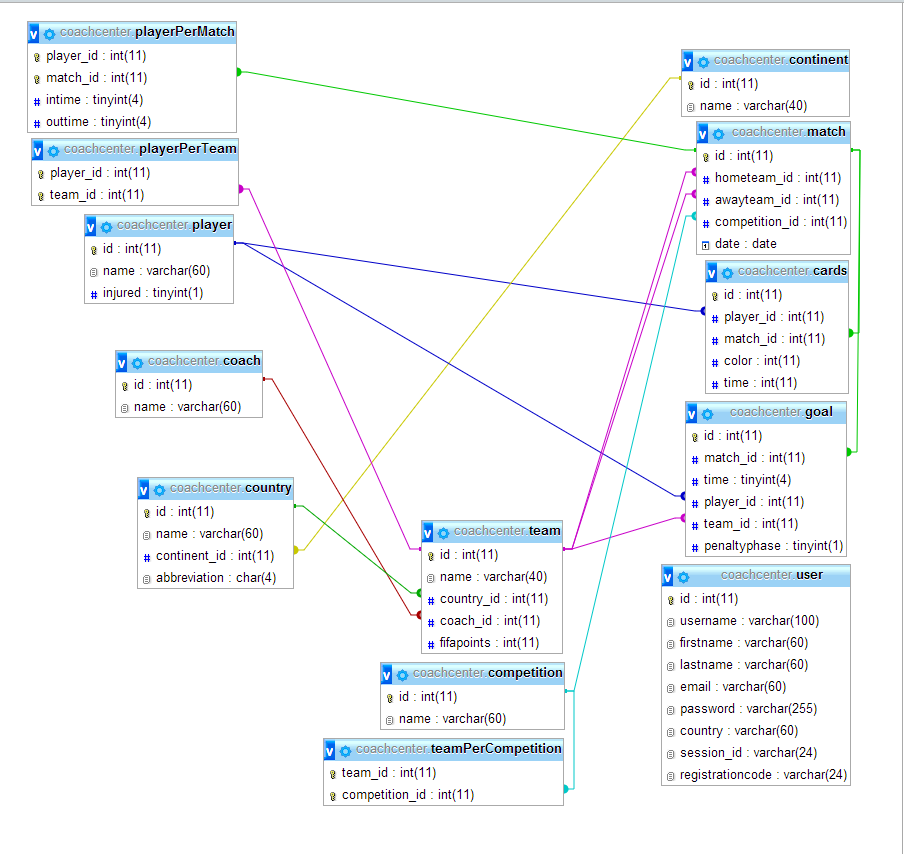
\includegraphics[width=90mm]{ER.png}
\caption{Onze database in ER-model}
\label{overflow}
\end{figure}

\end{document}
